%ARCHITETTURA APP ESTERNA
\subsection{Applicazione esterna alla piattaforma Grafana}
Per poter visualizzare la suddivisione delle componenti dell'applicazione esterna e le dipendenze che sussistono tra loro ad alto livello, viene riportato il diagramma dei Package in allegato nel file \textit{diagramma-package-app.png}.
	\subsubsection{Progettazione architetturale}
	Abbiamo deciso di utilizzare il design pattern\glosp architetturale Model-View-ViewModel (MVVM) perché si adatta bene alle due principali tecnologie che utilizzate: React ed Electron. In particolare, come si può vedere dalla figura seguente, la View scambia dei dati in modo asincrono con il ViewModel attraverso Electron e ciò permette di mantenere la View sempre aggiornata. Inoltre è presente la comunicazione tra ViewModel e Model che avviene con la richiesta di esecuzione delle operazioni da parte del ViewModel e la conseguente risposta da parte del Model. Anche questo scambio di messaggi è asincrono ed è implementato da un meccanismo di callback\glo.
	\mbox{}
	\begin{landscape}
		\begin{figure}
			\begin{figure} [H]
				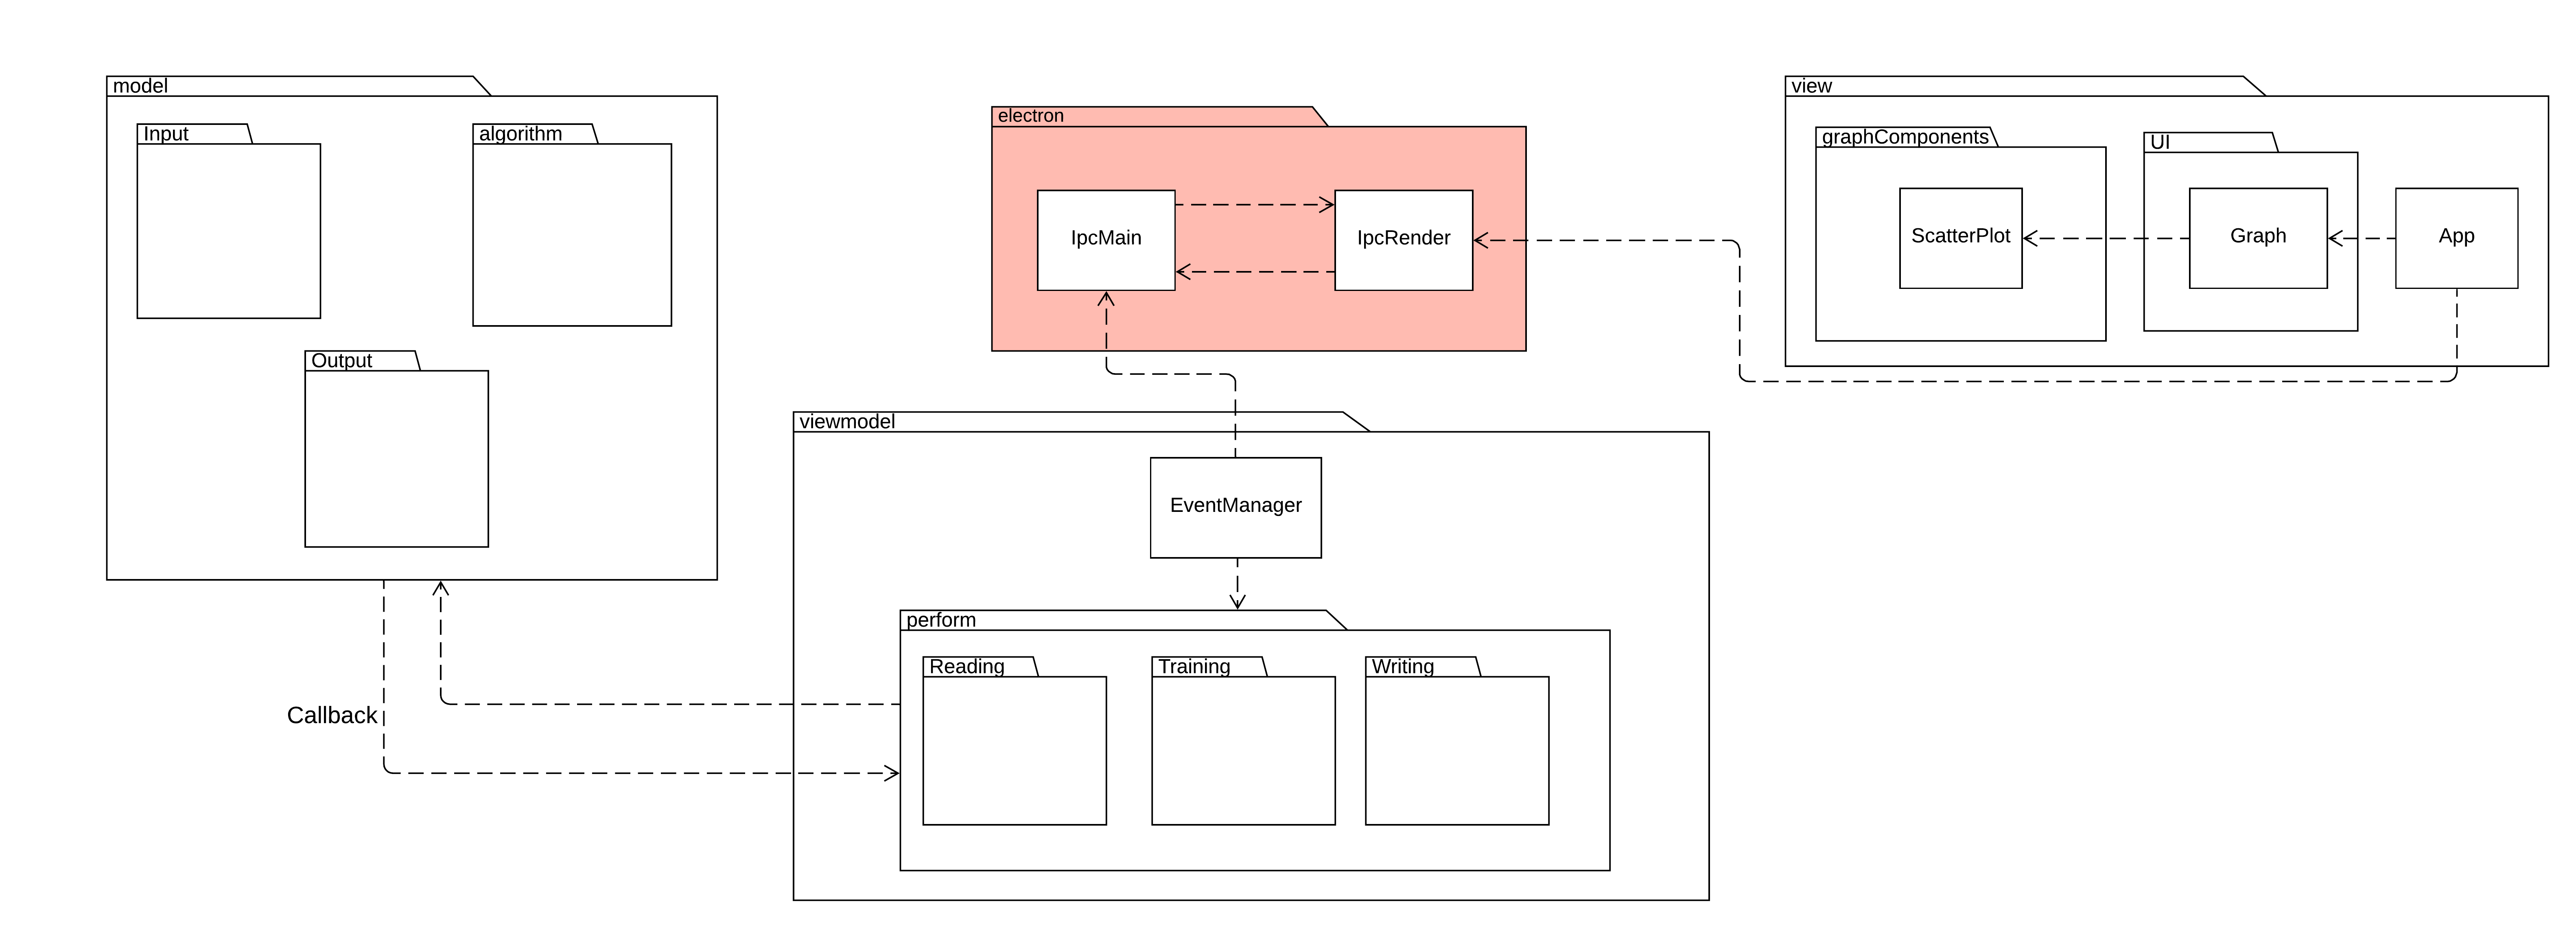
\includegraphics[width=\linewidth]{./img/Diagrammi/architettura-app.png}
				\caption{Diagramma dell'architettura dell'applicazione}
			\end{figure}
		\end{figure}
	\end{landscape}
	La nostra architettura è composta dai seguenti componenti: 
	\begin{itemize}
		\item \textbf{Model}: componente che gestisce la business logic\glosp dell'applicazione;
		\item \textbf{ViewModel}: componente che gestisce il binding\glosp tra View e Model con un meccanismo detto two-way-data-binding;
		\item \textbf{View}: componente che gestisce la presentazione dei dati attraverso React;
		\item \textbf{Electron}: componente esterno che gestisce lo scambio di messaggi asincrono tra View e ViewModel. È composto a sua volta da:
			\begin{itemize}
				\item \textbf{IpcMain}: Componente che permette di ricevere ed inviare segnali verso la View;
				\item \textbf{IpcRender}: Componente che permette di ricevere ed inviare segnali verso il ViewModel.
			\end{itemize}
	\end{itemize}
	\subsubsection{Progettazione di dettaglio}
		Di seguito viene descritta in dettaglio la progettazione dell'applicazione. In allegato viene fornito il file \textit{diagramma-classi-app.png} contenente l'intero diagramma delle classi.
		\paragraph{Model}
		I componenti principali del Model sono gli algoritmi di addestramento rappresentati dalle classi concrete \textit{SvmTrainer} ed \textit{RlTrainer} e le funzioni di lettura e scrittura dei file rappresentate dalle classi astratte rispettivamente \textit{Read} e \textit{Write}.
		Più in dettaglio fornisce le funzionalità di addestramento degli algoritmi di predizione Support Vector Machine\glosp lineare e regressione lineare\glosp con il corrispondente calcolo degli indici di qualità: Precision\glosp e Recall\glosp per il primo e Rq\glosp per il secondo. Per le operazioni con i file, invece, viene fornita la lettura da file CSV e JSON e la scrittura su file JSON.
		\paragraph*{SvmTrainer} \mbox{} \\[1mm]
		Questa classe, come detto in precedenza, ha lo scopo di addestrare l'algoritmo Support Vector Machine\glosp lineare sfruttando la clasese SVM della libreria nodeModules. \\
		Il campo dati che richiede un'ulteriore spiegazione è \textit{options} ovvero un array di stringhe che contiene le opzioni di esecuzione per l'algoritmo.
		Il metodo che invece necessita di un'ulteriore spiegazione è \textit{translateData()} in quanto prepara i dati nel formato adeguato all'addestramento. Inoltre suddivide i dati per il calcolo degli indici di qualità e per l'addestramento dell'algoritmo rispettivamente in 1/3 e 2/3 con una modalità pseudo-casuale per non porre vincoli all'utente in fase di inserimento. \\
		Questa classe ha una dipendenza verso il tipo \textbf{SvmData} che rappresenta la struttura del dato da dare in input ad una Svm\glo.
		\paragraph*{RlTrainer} \mbox{} \\[1mm]
		Questa classe, come detto in precedenza, ha lo scopo di addestrare l'algoritmo regressione lineare\glosp sfruttando la libreria LinearRegression. \\
		Il campo dati che richiede un'ulteriore spiegazione è \textit{options} ovvero un array di stringhe che contiene le opzioni di esecuzione per l'algoritmo.
		Il metodo che invece necessita di un'ulteriore spiegazione è \textit{translateData()} in quanto prepara i dati nel formato adeguato all'algoritmo. Inoltre suddivide i dati per il calcolo degli indici di qualità e per l'addestramento rispettivamente in 1/3 e 2/3 con una modalità pseudo-casuale per non porre vincoli all'utente in fase di inserimento. \\
		Questa classe ha una dipendenza verso il tipo \textbf{RlData} che rappresenta la struttura del dato da dare in input ad una Rl\glo.
		\paragraph*{Result} \mbox{} \\[1mm]
		Per definire il tipo risultato degli algoritmi di predizione abbiamo implementato l'interfaccia Result. Il contratto di questa interfaccia è composto da un solo metodo: \textit{toStringJson()}. Questo metodo ritorna un oggetto JSON contenente tutti i campi dati del risultato dell'addestramento sotto forma di stringa. In questo modo per ogni tipologia di algoritmo può essere definita una classe concreta che implementa Result e che contiene i propri dati. \\
		Nella nostra applicazione sono stati implementati \textbf{SvmResult} e \textbf{RlResult}:
		\mbox{}
		\begin{landscape}
			\begin{figure}
				\begin{figure} [H]
					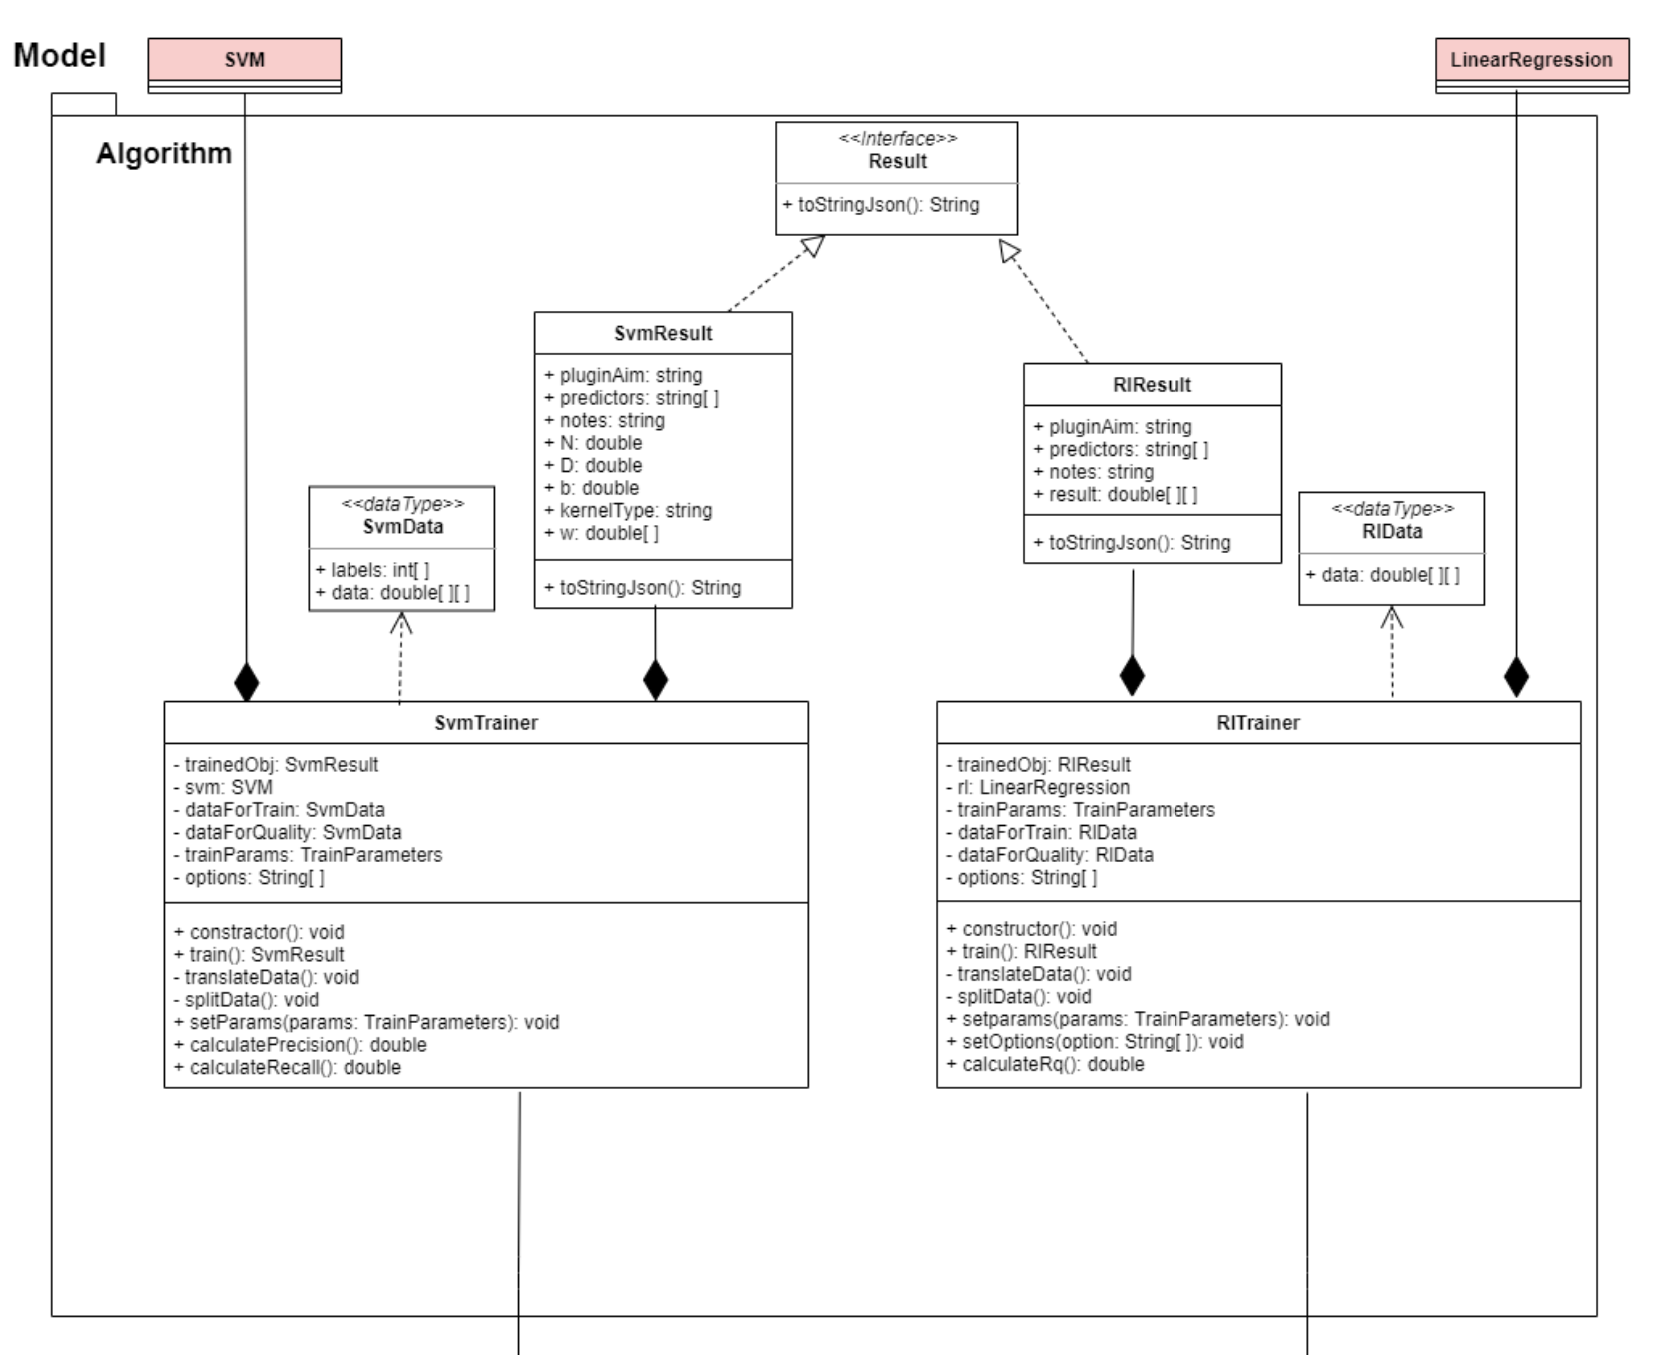
\includegraphics[width=\linewidth]{img/Diagrammi/algorithm-app.png}
					\caption{Diagramma delle classi per gli algoritmi nel Model}
				\end{figure}
			\end{figure}
		\end{landscape}
		\paragraph*{Read} \mbox{} \\[1mm]
		Abbiamo riscontrato nella gestione dell'input che, indipendentemente dalla tipologia di file ricevuto, l'algoritmo per eseguire la lettura di quest'ultimo ha uno scheletro comune. È stato quindi deciso di implementare il design pattern template method.
		La classe astratta \textit{Read} implementa il metodo \textit{ReadFile(path, callback)} che rappresenta la parte di interazione con il filesystem per la lettura da file, comune a qualsiasi tipologia. Inoltre fornisce il metodo astratto \textit{parser(data, callback)} che invece rappresenta la trasformazione del contenuto del file sulla base della sua estensione e, perciò, viene implementato nelle classi concrete che estendono \textit{Read}. Nel nostro caso esse sono \textit{ReadCsv} e \textit{ReadJson}.
		Infine per quanto riguarda \textit{ReadCsv}, ha una dipendenza di tipo composizione con la classe \textit{TrainParameters} che definisce la struttura dei parametri di addestramento letti dal file. Inoltre, a sua volta, ha una dipendenza di tipo composizione con il template di classe chiamato \textit{Series} che rappresenta il tipo vero e proprio dei parametri di addestramento. È stato definito come template in quanto non si vuole vincolare la tipologia di dato primitivo che contiene, permettendo di istanziarlo in base alle proprie necessità.
		\mbox{}
		%\begin{landscape}
			%\begin{figure}
				\begin{figure} [H]
					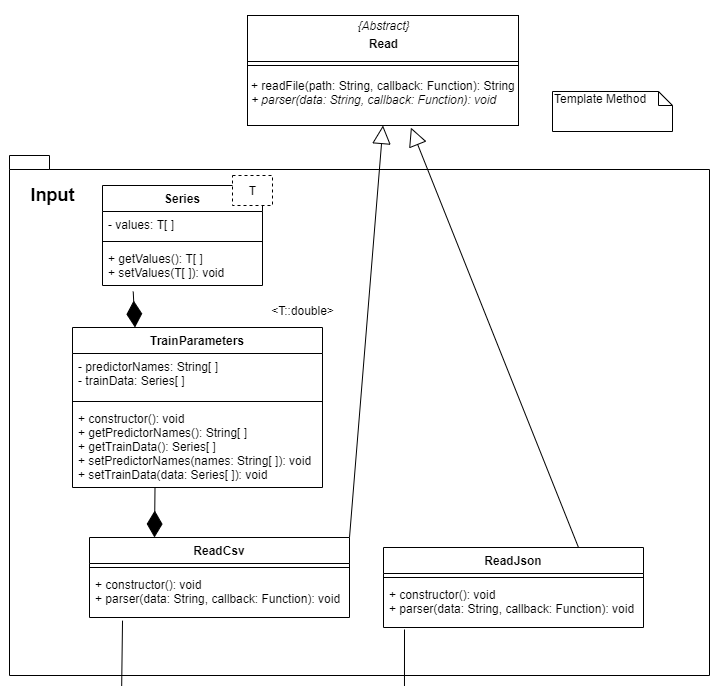
\includegraphics[width=\linewidth]{img/Diagrammi/read-app.png}
					\caption{Diagramma delle classi per la Read nel Model}
				\end{figure}
			%\end{figure}
		%\end{landscape}
		\paragraph*{Write} \mbox{} \\[1mm]
		Anche nella gestione dell'output abbiamo riscontrato che, indipendentemente dalla tipologia di file su cui scrivere, l'algoritmo per eseguire la scrittura ha uno scheletro comune. È stato quindi deciso di implementare il design pattern\glosp template method.
		La classe astratta \textit{Write} implementa il metodo \textit{writeToDisk(path, name, data, notes, callback)} che rappresenta la parte di interazione con il filesystem per la scrittura su file, comune a qualsiasi tipologia. Inoltre contiene il metodo astratto \textit{parser(data, callback)} che invece rappresenta la trasformazione dell'oggetto che vogliamo scrivere sul file nel formato corretto e che differisce dalla tipologia di file. Nel nostro caso abbiamo implementato la classe concreta \textit{WriteJson} che estende \textit{Write}.
		\mbox{}
		%\begin{landscape}
		%	\begin{figure}
				\begin{figure} [H]
					\begin{center}
						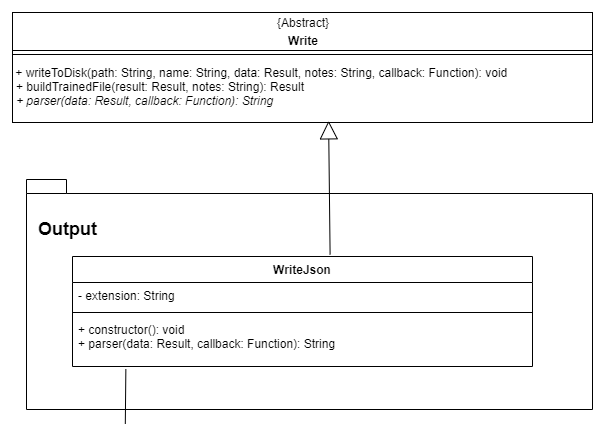
\includegraphics[width=120mm]{img/Diagrammi/write-app.png}
					\end{center}
					\caption{Diagramma delle classi per la Write nel Model}
				\end{figure}
		%	\end{figure}
		%\end{landscape}

		\paragraph{View} \mbox{} \\[1mm]
		La View è realizzata attraverso dei componenti di React contenuti nella classe principale \textit{App} attraverso una dipendenza di tipo composizione. Grazie all'estensione della classe \textit{Component} di React, otteniamo il metodo \textit{render()} che renderizza i componenti visualizzandoli nell'interfaccia utente.
		Infine per l'implementazione del grafico di addestramento, utilizziamo la libreria D3.
		\paragraph*{App}
		È la classe principale che orchestra tutti i componenti della View e che, attraverso Electron, comunica con la ViewModel. \\
		I campi dati che rappresentano i componenti dell'interfaccia utente sono:
		\begin{itemize}
			\item graph: è un oggetto di tipo Graph che rappresenta il grafico di visualizzazione dei dati e dell'addestramento;
			\item userNotes: è un oggetto di tipo UserNotes e rappresenta il componente grafico di inserimento delle note nel file di addestramento;
			\item modal: è un oggetto di tipo Modal e rappresenta il componente grafico di salvataggio di un file. A sua volta contiene un oggetto di tipo SaveFileName ?
			\item choose: è un oggetto di tipo Chooser che rappresenta il componente grafico che permette all'utente di scegliere i file nell'inserimento;
			\item paramModel: è un oggetto di tipo ParamModal che rappresenta il componente grafico di selezionamento dei valori durante il caricamento dei file csv.
		\end{itemize}
		\paragraph*{Graph}
		È la classe che gestisce il grafico ed ha una dipendenza di tipo composizione con le altre classi che ne rappresentano i componenti:
		\begin{itemize}
			\item ScatterPlot: è un oggetto di tipo RenderCircles e rappresenta...
			\item Grid:
			\item Axis: 
		\end{itemize}
		\mbox{}
		%\begin{landscape}
		%	\begin{figure}
				\begin{figure} [H]
					\begin{center}
						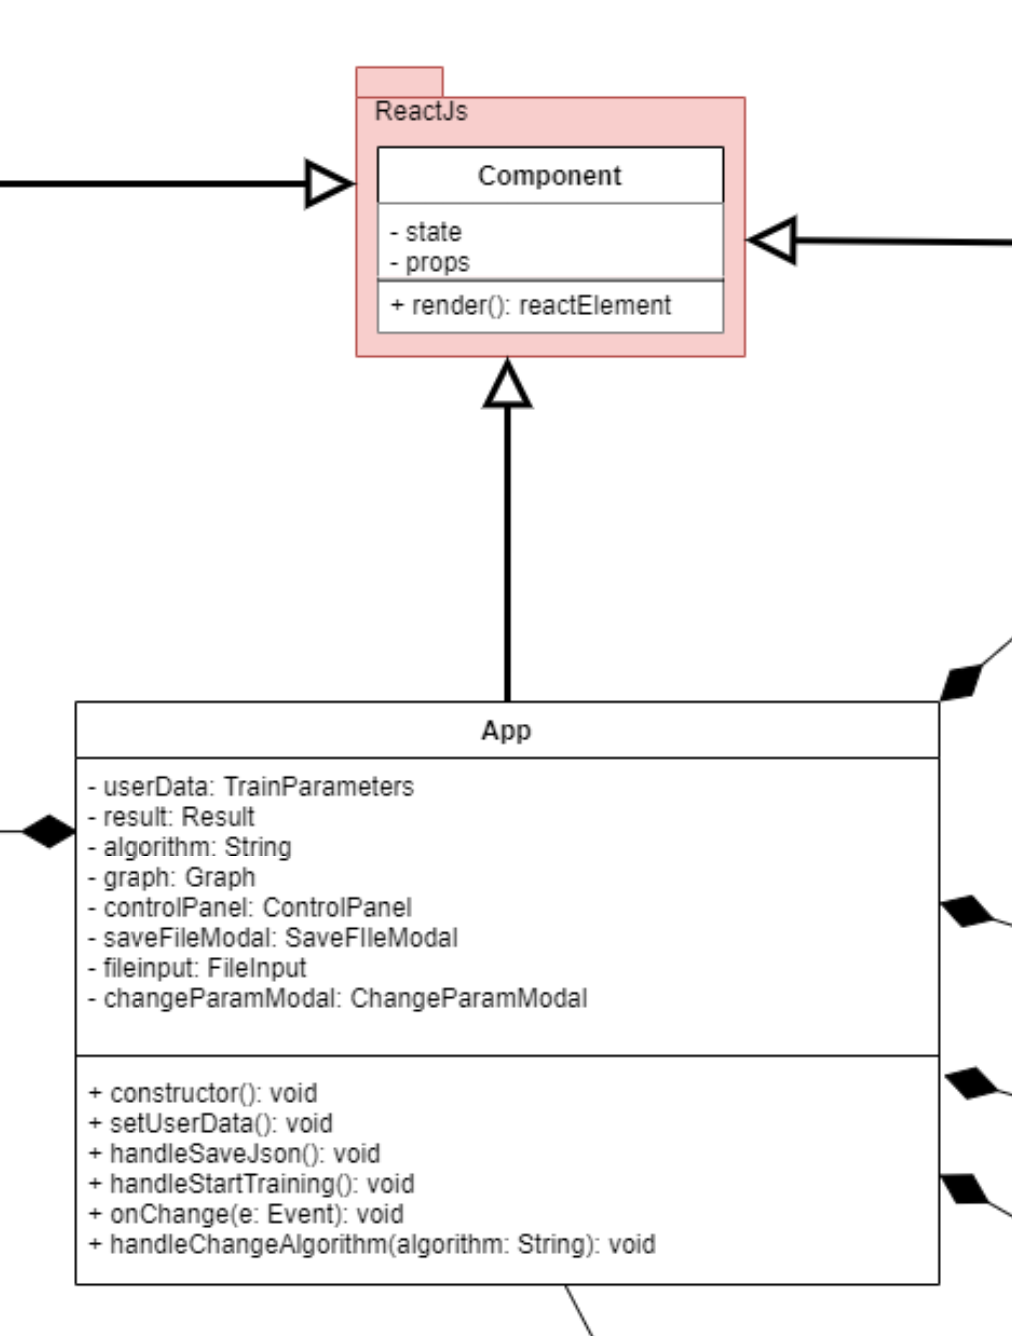
\includegraphics[width=100mm]{img/Diagrammi/view-app.png}
					\end{center}
					\caption{Diagramma delle classi della View}
				\end{figure}
		%	\end{figure}
		%\end{landscape}
	
		\paragraph{ViewModel} \mbox{} \\[1mm]
		La ViewModel contiene i dati da visualizzare nella vista e le trasformazioni per richiamare le operazioni da eseguire nel modello.
		In particolare è legato alla View tramite Electron che gestisce la loro comunicazione in modo asincrono appoggiandosi al nostro componente \textit{EventManager} e al Model attraverso il meccanismo asincrono di callback.
		Abbiamo riscontrato la necessità di implementare il design pattern\glosp strategy in tre casi diversi:
		\paragraph*{Train} \mbox{} \\[1mm]
		All'interno di questo package descriviamo le classi che eseguono le trasformazioni necessarie per eseguire l'addestramento richiamando \textit{SvmTrainer} e \textit{RlTrainer} ma anche forniscono i risultati alla View per la visualizzazione. Sono le seguenti:
		\begin{itemize}
			\item \textbf{ProcessTraining}: è una classe concreta che rappresenta il context. In essa viene scelto quale algoritmo addestrare sulla base dei dati ricevuti ed ha una dipendenza di tipo aggregazione dall'interfaccia \textit{PerformTraining};
			\item \textbf{PerformTraining}: è un'interfaccia che rappresenta la strategia astratta. Essa definisce il contratto da rispettare per le classi che implementano il process degli algoritmi di addestramento;
			\item \textbf{PerformTrainingSvm}: è una classe concreta che implementa \textit{PerformTraining} e rappresenta il componente che esegue la trasformazione ed il controllo dei dati per richiamare correttamente l'algortimo di addestramento SVM\glosp nel Model.
			\item \textbf{PerformTrainingRl}: è una classe concreta che implementa \textit{PerformTraining} e rappresenta il componente che esegue la trasformazione ed il controllo dei dati per richiamare correttamente l'algortimo di addestramento RL\glosp nel Model.
		\end{itemize}
		\mbox{}
		\begin{landscape}
			\begin{figure}
				\begin{figure} [H]
					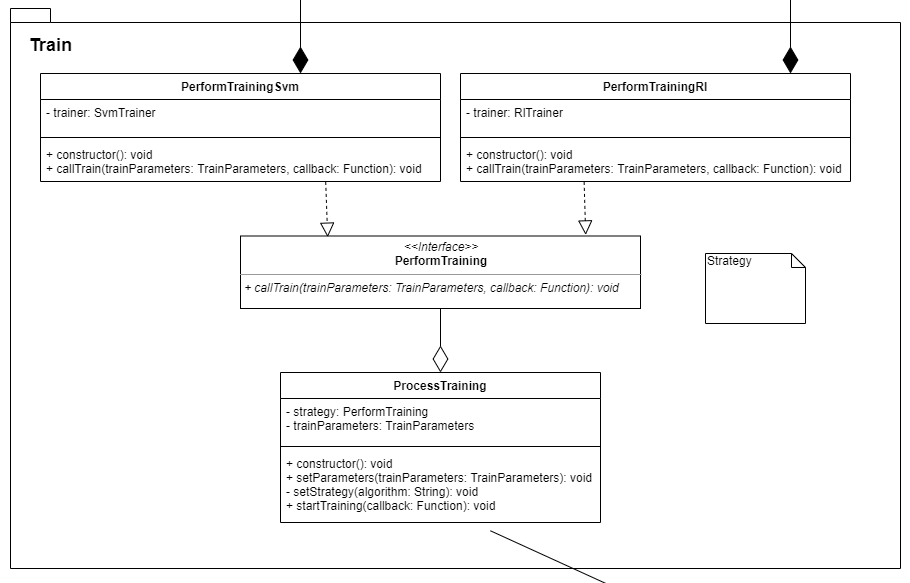
\includegraphics[width=\linewidth]{img/Diagrammi/ViewModel-train-app.png}
					\caption{Diagramma delle classi per il training nel ViewModel}
				\end{figure}
			\end{figure}
		\end{landscape}
		\paragraph*{Diagramma di sequenza} \mbox{} \\[1mm]
		Per spiegare meglio l'insieme di azioni compiute al fine di processare i dati per eseguire l'addestramento degli algoritmi, illustriamo un diagramma di sequenza che prende in esame SVM\glo. Per gli altri algoritmi il procedimento è simile.
		\mbox{}
		\begin{landscape}
			\begin{figure}
				\begin{figure} [H]
					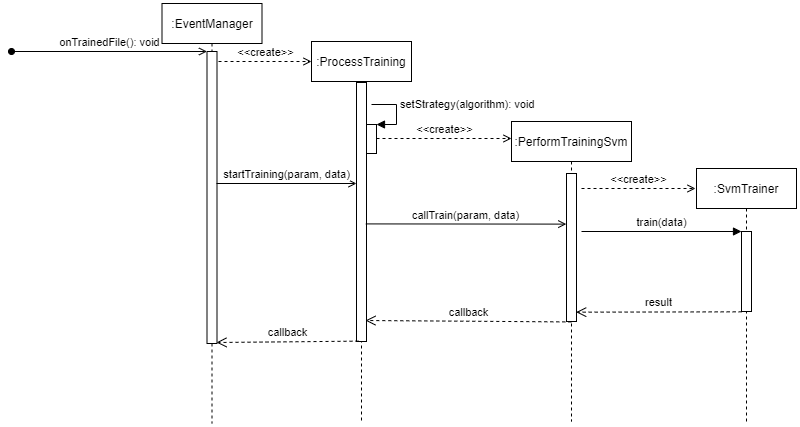
\includegraphics[width=\linewidth]{img/Diagrammi/ds-app.png}
					\caption{Diagramma di sequenza di processo dei dati per SVM}
				\end{figure}
			\end{figure}
		\end{landscape}
		\paragraph*{Read} \mbox{} \\[1mm]
		All'interno di questo package descriviamo le classi che eseguono le trasformazioni necessarie per eseguire la lettura da file, csv e json nel nostro caso, e che forniscono i risultati visualizzare successivamente sulla View.
		\begin{itemize}
			\item \textbf{ProcessReading}: è una classe concreta che rappresenta il context. In essa viene scelta la tipologia di file da leggere sulla base dei dati ricevuti ed ha una dipendenza di tipo aggregazione dall'interfaccia \textit{PerformReading};
			\item \textbf{PerformReading}: è un'interfaccia che rappresenta la strategia astratta. Essa definisce il contratto da rispettare per le classi che implementano la lettura da file;
			\item \textbf{PerformReadingCsv}: è una classe concreta che implementa \textit{PerformReading} e rappresenta il componente che esegue le trasformazioni necessarie per richiamare la correttamente l'algoritmo di lettura di un file Csv del Model;
			\item \textbf{PerformReadingJSon}: è una classe concreta che implementa \textit{PerformReading} e rappresenta il componente ch esegue le trasformazioni necessarie per richiamare la correttamente l'algoritmo di lettura di un file Json del Model.
		\end{itemize}
		\mbox{}
		%\begin{landscape}
		%	\begin{figure}
				\begin{figure} [H]
					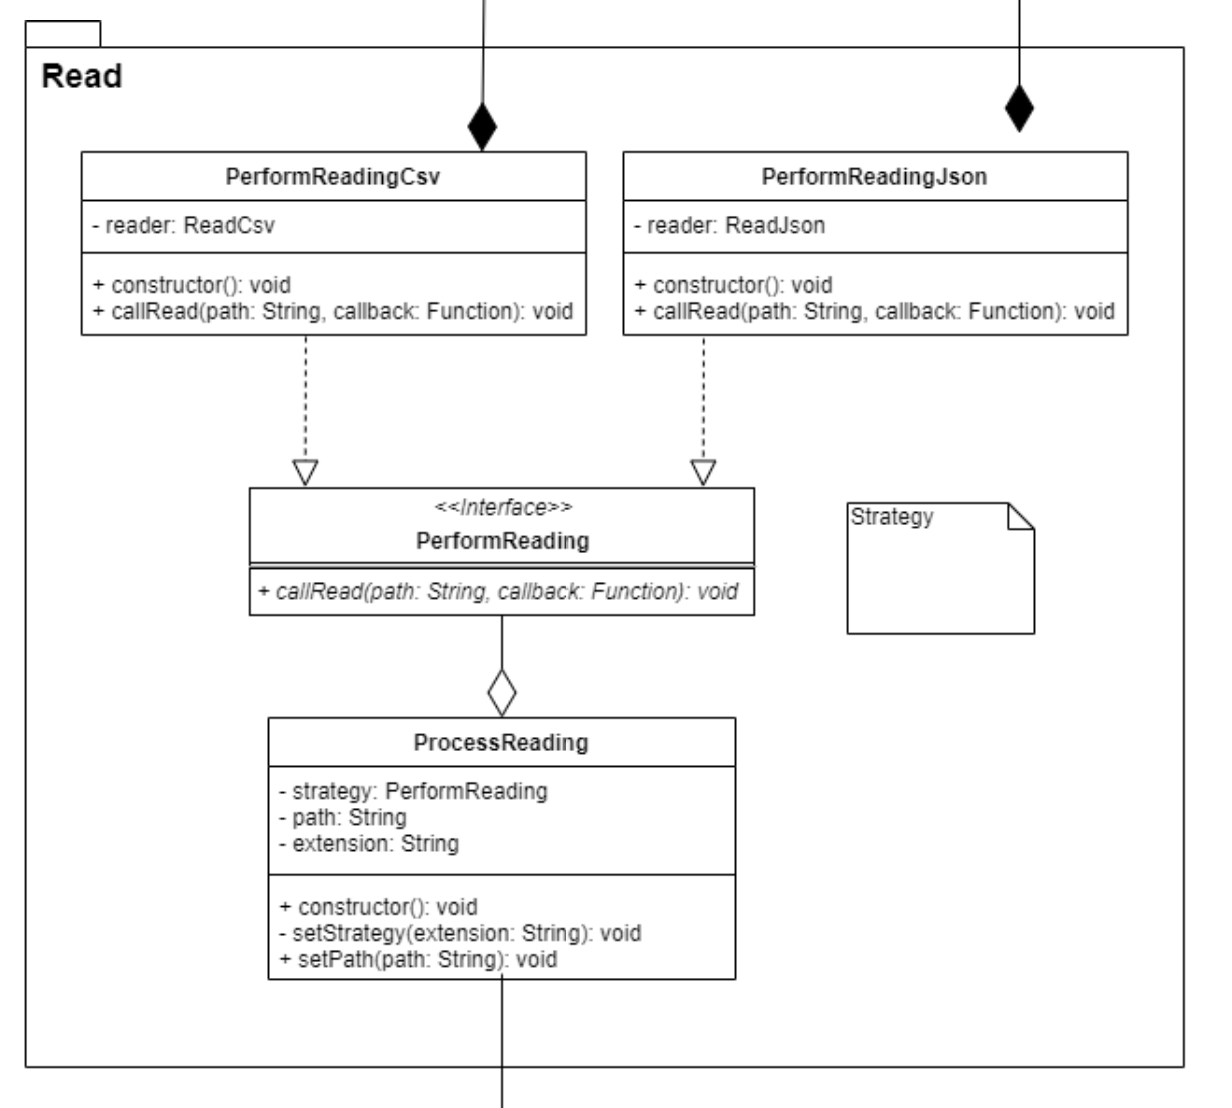
\includegraphics[width=\linewidth]{img/Diagrammi/ViewModel-read-app.png}
					\caption{Diagramma delle classi per la Read nel ViewModel}
				\end{figure}
		%	\end{figure}
		%\end{landscape}
		\paragraph*{Writing} \mbox{} \\[1mm]
		All'interno di questo package descriviamo le classi che eseguono le trasformazioni necessarie per eseguire la scrittura su file, json nel nostro caso, e che forniscono i risultati visualizzare successivamente sulla View.
		\begin{itemize}
			\item \textbf{ProcessWriting}: è una classe concreta che rappresenta il context. in essa viene scelta la tipologia di file su cui scrivere in base ai dati ricevuti ed ha una dipendenza di tipo aggregazione dall'interfaccia \textit{PerformWriting};
			\item \textbf{PerformWriting}: è un'interfaccia che rappresenta la strategia astratta. Essa definisce il contratto da rispettare per le classi che implementano la lettura da file;
			\item \textbf{PerformWritingJson}: è una classe concreta che implementa \textit{PerformWriting} e rappresenta il componente che esegue le trasformazioni necessarie per richiamare correttamente l'algoritmo di scrittura di un file Json del Model. Al suo interno ha un campo dati di tipo FileInfo che definisce tutte le informazioni ricavate dal file.
		\end{itemize}
		\mbox{}
		%\begin{landscape}
		%	\begin{figure}
				\begin{figure} [H]
					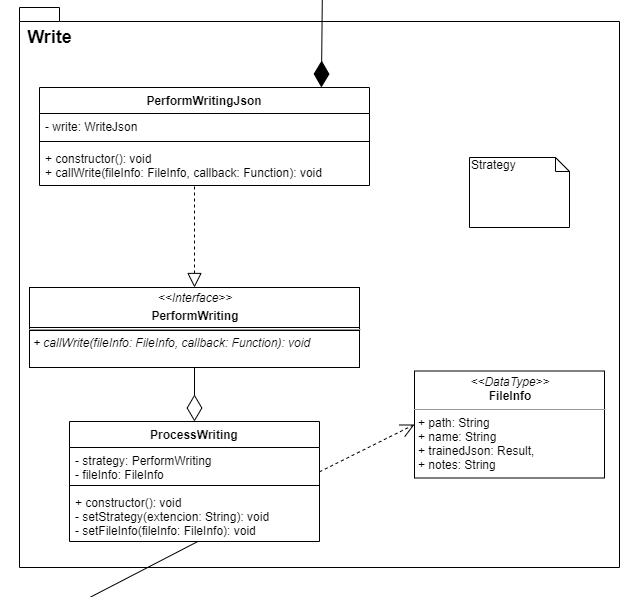
\includegraphics[width=\linewidth]{img/Diagrammi/ViewModel-write-app.png}
					\caption{Diagramma delle classi per la Write nel ViewModel}
				\end{figure}
		%	\end{figure}
		%\end{landscape}
		
